% !TEX root = ../ausarbeitung.tex

\chapter{Herangehensweise}

Im Hauptteil beschreiben Sie Ihre praktische Arbeit. Code gehört normalerweise nicht in eine Ausarbeitung. Ausnahmen sind Algorithmen, die für Sie wichtig waren (dann in möglichst übersichtlichem Pseudo-Code). Kleine Code-Stücke können auch zur Illustration oder als Beispiel eingebaut werden. Längere Code-Stücke können im Anhang untergebracht werden. Sie sollten jedoch nicht den gesamten Code im Anhang abdrucken. Ihren Code geben Sie bitte dennoch mit ab, am besten auf einer CD.

Der Detailgrad sollte so sein, dass ein Leser die gleiche Arbeit noch einmal nachimplementieren könnte. Insbesondere sollten alle Parameter, von denen die Funktionsweise des Systems abhängt, explizit genannt sein. Bei der Evaluation muss bei jedem Versuch angegeben werden, mit welchen Parametern gearbeitet wird.


\hfil\rule{0.4\textwidth}{0.4pt}

\section{Einführung in \LaTeX}
Wenn Sie dieses Template gefunden haben, werden Sie schon erkannt haben, dass \LaTeX\ nicht ganz unwichtig ist. Falls Sie noch kaum oder keine Erfahrung damit haben, bietet sich der Kurs \qq{Einführung in \LaTeX} von Thorsten Nagel an. Er findet meistens mehrmals im Semester statt, die genauen Termine entnehmen Sie bitte dem Vorlesungsverzeichnis. Das Skript zu diesem Kurs ist online erhältlich \cite{thorstennagel2015} und enthält noch viele weitere Informationen, die in der folgenden Kurzzusammenfassung nicht berücksichtigt werden konnten.

\section{Sinnvolle Programme}
Falls Sie \verb|.tex|-Dateien nicht unbedingt in einem normalen Texteditor schreiben und auf der Kommandozeile kompilieren möchten, bietet sich ein spezieller \LaTeX-Editor wie z.B. TeXstudio \cite{texstudio} an.

\section{Wichtige \LaTeX-Befehle}
\subsection{Textgliederung}
Mit dem Befehl \verb|\section{Überschrift}| lässt sich ein neuer Abschnitt beginnen, der automatisch nummeriert und im \hyperref[toc]{Inhaltsverzeichnis} eingetragen wird.
Gleiches gilt für einen Unterabschnitt, der mit \verb|\subsection{Unterüberschrift}| begonnen wird.

\LaTeX\ bietet noch weitere Gliederungsebenen bis hin zum Unterabsatz, die aber standardmäßig nicht mehr nummeriert werden und standardmäßig auch nicht im Inhaltsverzeichnis auftauchen. Im Normalfall sind diese aber nicht unbedingt nötig.
\subsubsection{Unterunterüberschrift}
\paragraph{Absatztitel} Absatztext
\subparagraph{Unterabsatz} Absatztext

Um in der PDF-Datei einen Zeilenumbruch zu erhalten, schreiben Sie im Quelltext \verb|\\|, für einen neuen Absatz lassen Sie eine Zeile frei. Ein einzelner Zeilenumbruch im Quelltext hat keine Auswirkungen.

\section{Formatierungen, Listen, Aufzählungen}
Um die \LaTeX-Befehle für die folgenden Formatierungen zu sehen, schauen Sie sich einfach den Quellcode an.

Text kann man \textbf{fett} oder \textit{kursiv} schreiben. Sie können Text auch explizit \emph{betonen}, was dann ebenfalls kursiv dargestellt wird.

Listen sind natürlich auch möglich, diese können beliebig verschachtelt werden.
\begin{itemize}
\item Listenpunkt 1
\item Listenpunkt 2
\begin{itemize}
\item Unterpunkt
\end{itemize}
\end{itemize}

Oder eine nummerierte Aufzählung:
\begin{enumerate}
\item Listenpunkt 1
\item Listenpunkt 2
\begin{enumerate}
\item Unterpunkt
\end{enumerate}
\end{enumerate}

\section{Tabellen}
Tabellen können wie folgt erstellt werden (siehe \autoref{tab:tabelle-1}):
\begin{table}[htb]
\centering
\caption{Formatierungsparameter zur Spaltenausrichtung in Tabellen\label{tab:tabelle-1}}
\begin{tabular}{l|p{3.5cm}lcr}
	                     & \textbf{Spalte 1}                   & \textbf{Spalte 2} & \textbf{Spalte 3} & \textbf{Spalte 4} \\ \hline
	\textbf{Parameter}   & \verb|p{3.5cm}|                     & \verb|l|          &     \verb|c|      &          \verb|r| \\
	\textbf{Ausrichtung} & linksbündig mit vorgegebener Breite & linksbündig       &     zentriert     &      rechtsbündig
\end{tabular}
\end{table}

Für \qq{schönere} Tabellen empfiehlt sich das \LaTeX-Paket \verb|booktabs|, das in der Präambel mit \verb|\usepackage{booktabs}| eingebunden werden kann. Insbesondere die zugehörige Anleitung \cite{booktabs} ist lesenswert, da sie recht einfach vermittelt, was eine \qq{schöne} Tabelle ausmacht.

\section{Mathematische Gleichungen}
Gleichungen oder sonstige Formeln im Fließtext, wie z.B. $f(x)=ax+b$, können Sie einfach in Dollarzeichen \verb|$...$| einfassen. Größere Formeln können auch in einer eigenen Zeile stehen:
\begin{displaymath}
g(x) = \frac{1}{2\pi\sigma}\cdot e^{-\frac{(x-\mu)^2}{2\sigma^2}}
\end{displaymath}
Falls Sie in Ihrer Ausarbeitung viel Mathematik benötigen, lohnt sich auch ein Blick auf das \LaTeX-Paket \verb|amsmath|.
\section{Abbildungen}
Abbildungen und Diagramme können Sie direkt in einer \verb|.tex|-Datei \qq{malen}. Dazu bietet TikZ viele Möglichkeiten, eine Grafik mit Text zu beschreiben. Falls Sie nicht jeden Strich in einem Diagramm selbst definieren wollen, bietet sich die Verwendung von Pgfplots in Form der \verb|axis|-Umgebung an, wie in \autoref{fig:diagramm} gezeigt.

Falls Sie sich näher mit der Materie beschäftigen wollen, bietet sich das Manual für TikZ und PGF\cite{pgfmanual} an. Dieses Dokument ist zwar sehr umfangreich (über 1000 Seiten), bietet aber viele gut erklärte Beispiele, auch und gerade für den Einstieg.

Die folgenden Abbildungen wurden in jeweils eine \verb|figure|-Umgebung gesteckt. Diese erzeugt eine \qq{floatende} Abbildung, die von \LaTeX\ automatisch an einer \qq{geeigneten} Stelle platziert wird, also nicht zwangsläufig dort, wo sie im Quelltext definiert wurde. Wenn Sie der Abbildung eine \verb|\caption{...}| und ein \verb|\label{key}| verpassen, können Sie über dieses Label im Text per \verb|\ref{key}| oder \verb|\autoref{key}| darauf verweisen. Bei ersterem wird nur die Nummer (\qq{\ref{fig:diagramm}}), bei letzterem zusätzlich noch der Typ (\qq{\autoref{fig:diagramm}}) ausgegeben. Analog zur \verb|figure|-Umgebung wurde oben für die Tabelle die \verb|table|-Umgebung verwendet.
\begin{figure}[htb]
\centering
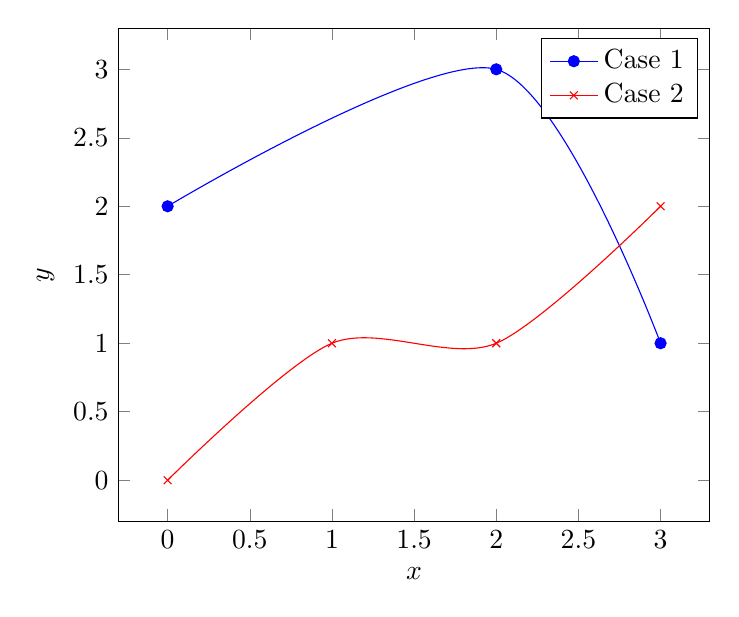
\begin{tikzpicture}
  \begin{axis}[xlabel=$x$,ylabel=$y$,width=0.75\textwidth]
    \addplot[smooth,mark=*,blue] plot coordinates {
        (0,2)
        (2,3)
        (3,1)
    };
    \addlegendentry{Case 1}

    \addplot[smooth,color=red,mark=x] plot coordinates {
            (0,0)
            (1,1)
            (2,1)
            (3,2)
        };
    \addlegendentry{Case 2}
  \end{axis}
\end{tikzpicture}
\caption{Diagramm aus den TikZ-Beispielen für Pgfplots\label{fig:diagramm}}
\end{figure}

Falls Sie eine Abbildung schon als separate Datei (z.B. im PDF-Format) vorliegen haben, können Sie diese mit \verb|\includegraphics{}| und dem Dateinamen einbinden, wie in \autoref{fig:smileys} geschehen. Dabei wird in den in der Präambel mit \verb|\graphicspath{...}| vorgegebenen Pfaden gesucht. Die Dateiendung wird automatisch \qq{erraten}, wenn sie nicht angegeben wird.
\begin{figure}[htb]
	\centering
	
\includegraphics[width=0.75\textwidth]{smileys}
	\caption{Darstellung des Wohlbefindens anhand von Smileys\label{fig:smileys}}
\end{figure}
